% =====================================================================================================
%  Radiology: Artificial Intelligence -- Original Research (concise draft v2, 2026-09-22)
%  ONE manuscript: level identification from operating-room C-arm shots alone, and the physics-parameterised
%  synthetic corpus that makes one detector work on every C-arm. Reader: a neurosurgeon fluent in AI.
%  Every number is a macro from claims.tex (tools/claims_fill.py <- docs/RSNAI_CLAIMS.json <- result JSONs).
%  \todo{} marks a result whose box in docs/RSNAI_PLAN.md is not yet ticked. Nothing is typed from memory.
% =====================================================================================================
\documentclass[11pt,letterpaper]{article}
\usepackage[margin=1in]{geometry}
\usepackage{setspace}\doublespacing
\usepackage{times}
\usepackage{graphicx,booktabs,array,amsmath,amssymb,xcolor,microtype,lineno}
\usepackage[labelfont=bf,font=small]{caption}
\usepackage[numbers,sort&compress]{natbib}
\usepackage[hidelinks]{hyperref}
\linenumbers
\graphicspath{{figures/}{../../SchwingNet/figures/}}
% GENERATED by tools/claims_fill.py from docs/RSNAI_CLAIMS.json -- do not edit; add or fix a claim in the ledger.

\newcommand{\clCarmCvFiveLatWholeExact}{98.2}  % C-ArmLSpine lateral, whole frame: exact level, five-fold CV over 141 cases / 617 vertebrae [docs/carmlspine_cv5_mixed_2026-09-21.json :: det/LAT/kfull.exact]
\newcommand{\clCarmCvFiveLatWholeCiLo}{95.7}  % its case-bootstrap 95 % CI, lower [docs/carmlspine_cv5_mixed_2026-09-21.json :: det/LAT/kfull.exact_ci.0]
\newcommand{\clCarmCvFiveApWholeExact}{96.7}  % C-ArmLSpine AP, whole frame: exact level, five-fold CV [docs/carmlspine_cv5_mixed_2026-09-21.json :: det/AP/kfull.exact]
\newcommand{\clCarmCvFiveLatKFiveExact}{97.0}  % C-ArmLSpine lateral, five vertebrae in the field: exact level [docs/carmlspine_cv5_mixed_2026-09-21.json :: det/LAT/k5.exact]
\newcommand{\clCarmCvFiveLatKThreeExact}{92.9}  % C-ArmLSpine lateral, three vertebrae in the field: exact level [docs/carmlspine_cv5_mixed_2026-09-21.json :: det/LAT/k3.exact]
\newcommand{\clCarmCvFiveLatKOneExact}{72.8}  % C-ArmLSpine lateral, one vertebra in the field: exact level [docs/carmlspine_cv5_mixed_2026-09-21.json :: det/LAT/k1.exact]
\newcommand{\clCarmZeroshotApWholeExact}{37.9}  % zero-shot level model (no C-ArmLSpine training), AP whole frame: exact level [docs/carmlspine_zeroshot2_pooled_all_2026-09-21.json :: det/AP/kfull.exact]
\newcommand{\clCarmZeroshotLatWholeExact}{96.3}  % zero-shot level model, lateral whole frame: exact level [docs/carmlspine_zeroshot2_pooled_all_2026-09-21.json :: det/LAT/kfull.exact]
\newcommand{\clLodoCarmHeldoutVertOutlineZeroTwoFive}{90.6}  % detector trained on COBRA + DeepFluoro real frames, C-ArmLSpine held out: vertebra recall, whole-vertebra outline truth, IoU 0.5, conf 0.25 [/rs/rs_grp_oschome/go2432/data/or_ready/lodo/rescore_outline.json :: lodo_carm__carm_test.recall.outline.8]
\newcommand{\clLodoCarmHeldoutVertBodyZeroTwoFive}{5.2}  % the same predictions against vertebral-body truth (the convention mismatch) [/rs/rs_grp_oschome/go2432/data/or_ready/lodo/rescore_outline.json :: lodo_carm__carm_test.recall.body.8]
\newcommand{\clLodoCarmHeldoutVertCentreZeroTwoFive}{90.9}  % the same predictions under the mutual-centre rule [/rs/rs_grp_oschome/go2432/data/or_ready/lodo/rescore_outline.json :: lodo_carm__carm_test.recall.centre.8]
\newcommand{\clPooledCarmVertOutlineZeroTwoFiveControl}{40.8}  % same-device pooled detector on C-ArmLSpine under outline truth (control: must fall) [/rs/rs_grp_oschome/go2432/data/or_ready/lodo/rescore_outline.json :: pooled__carm_test.recall.outline.8]
\newcommand{\clCardCiosRTwoHeldout}{0.905}  % Siemens Cios Fusion card: held-out R2 of the nine-term physics model [docs/devices/cios_fusion.json :: physics_terms.held_out_r2_median]
\newcommand{\clCardCiosRTwoBaseline}{0.899}  % Siemens Cios Fusion card: held-out R2 of uncalibrated physics + linear match [docs/devices/cios_fusion.json :: physics_terms.baseline_r2_median]
\newcommand{\clCardPulseraRTwoHeldout}{0.952}  % Philips BV Pulsera card: held-out R2 [docs/devices/bv_pulsera.json :: physics_terms.held_out_r2_median]
\newcommand{\clCardPulseraRTwoBaseline}{0.917}  % Philips BV Pulsera card: baseline R2 [docs/devices/bv_pulsera.json :: physics_terms.baseline_r2_median]
\newcommand{\clCardPulseraTypicalityNineNine}{80.2}  % Philips BV Pulsera: share of held-out frames typical under the sampler (99th percentile), photons-only per-frame refit [docs/devices/bv_pulsera.json :: distribution.coverage.typicality_99]
\newcommand{\clManifoldOverlapCiosElekta}{0.018}  % Bhattacharyya overlap of the Cios Fusion and Elekta XVI real-frame densities in the 3-D statistics space [/rs/rs_grp_oschome/go2432/data/or_ready/manifold/overlap.json :: overlap_bhattacharyya.cios_fusion|elekta_xvi]
\newcommand{\clManifoldOverlapSurgioFilm}{0.289}  % Bhattacharyya overlap Surgio-B51 vs plain film (the largest) [/rs/rs_grp_oschome/go2432/data/or_ready/manifold/overlap.json :: overlap_bhattacharyya.film|surgio_b51_dr]
\newcommand{\clManifoldNReal}{1{,}861}  % real frames embedded [/rs/rs_grp_oschome/go2432/data/or_ready/manifold/overlap.json :: n_real]
\newcommand{\clCardCiosTypicalityNineNine}{10.1}  % Siemens Cios Fusion: typicality_99 after the photons-only per-frame refit (six cadavers as folds) [docs/devices/cios_fusion.json :: distribution.coverage.typicality_99]
\newcommand{\clCardElektaTypicalityNineNine}{84.8}  % Elekta XVI: typicality_99 after the photons-only per-frame refit [docs/devices/elekta_xvi.json :: distribution.coverage.typicality_99]
\newcommand{\clCardElektaRTwoHeldout}{0.974}  % Elekta XVI card: held-out R2 [docs/devices/elekta_xvi.json :: physics_terms.held_out_r2_median]
\newcommand{\clCardElektaRTwoBaseline}{0.964}  % Elekta XVI card: baseline R2 [docs/devices/elekta_xvi.json :: physics_terms.baseline_r2_median]
\newcommand{\clCardCiosPhotonsMedianPerFitPx}{5{,}943}  % Siemens Cios Fusion: median quantum count per 0.776 mm fit pixel, photons-only per-frame refit [docs/devices/cios_fusion.json :: physics_terms.photons_per_fit_px.median]
\newcommand{\clCarmCvFiveFrames}{148}  % C-ArmLSpine five-fold CV: lateral whole frames scored (one per case) [docs/carmlspine_cv5_mixed_2026-09-21.json :: det/LAT/kfull.frames]
\newcommand{\clCarmCvFiveLatWholeCases}{141}  % C-ArmLSpine lateral whole frames: cases with at least one scorable vertebra [docs/carmlspine_cv5_mixed_2026-09-21.json :: det/LAT/kfull.cases]
\newcommand{\clCarmCvFiveLatWholeVertebrae}{617}  % C-ArmLSpine lateral whole frames: scorable vertebrae (both segmentation tools agree) [docs/carmlspine_cv5_mixed_2026-09-21.json :: det/LAT/kfull.vertebrae]
\newcommand{\clCarmCvFiveLatWholeWithinOne}{100}  % C-ArmLSpine lateral whole frames: level within one [docs/carmlspine_cv5_mixed_2026-09-21.json :: det/LAT/kfull.within1]
\newcommand{\clCarmCvFiveApWholeWithinOne}{100}  % C-ArmLSpine AP whole frames: level within one [docs/carmlspine_cv5_mixed_2026-09-21.json :: det/AP/kfull.within1]
\newcommand{\clCarmCvFiveLatKOneWithinOne}{90.2}  % C-ArmLSpine lateral, one vertebra in the field: level within one [docs/carmlspine_cv5_mixed_2026-09-21.json :: det/LAT/k1.within1]
\newcommand{\clLodoCarmHeldoutSacrumZeroTwoFive}{83.9}  % detector trained on COBRA + DeepFluoro real frames, C-ArmLSpine held out: sacrum found, outline truth, IoU 0.5, conf 0.25 [/rs/rs_grp_oschome/go2432/data/or_ready/lodo/rescore_outline.json :: lodo_carm__carm_test.sacrum_found.outline.8]
\newcommand{\clRenderDetRealFilmRecall}{71.7}  % detector trained on 6,650 renders and no real image (anchor_det_v1), per-body recall on real radiographs (films_drr_buucorr), conf 0.05 [/wsu/home/go/go24/go2432/model_night/render_detector/render_det_on_real_films.json :: by_conf.0.05.recall]
\newcommand{\clFilmDetRealFilmRecall}{99.1}  % same architecture trained on real film (detect_v5z_final), per-body recall on the same real radiographs, conf 0.05 [/wsu/home/go/go24/go2432/model_night/render_detector/film_det_on_real_films.json :: by_conf.0.05.recall]
\newcommand{\clRenderDetRendersRecall}{93.5}  % render-trained detector on renders (its own domain, ctsp_drr), per-body recall, conf 0.05 [/wsu/home/go/go24/go2432/model_night/render_detector/render_det_on_renders.json :: by_conf.0.05.recall]
\newcommand{\clRenderDetRealFilmBodies}{233}  % real-radiograph test for the render/film detector comparison: vertebral bodies [/wsu/home/go/go24/go2432/model_night/render_detector/render_det_on_real_films.json :: by_conf.0.05.bodies]
\newcommand{\clRenderDetRealFilmFrames}{71}  % real-radiograph test for the render/film detector comparison: frames [/wsu/home/go/go24/go2432/model_night/render_detector/render_det_on_real_films.json :: by_conf.0.05.frames]
\newcommand{\clRenderDetRealFilmSpines}{25}  % real-radiograph test for the render/film detector comparison: spines [/wsu/home/go/go24/go2432/model_night/render_detector/render_det_on_real_films.json :: by_conf.0.05.spines]
\newcommand{\clFilmNamingCsxaRandom}{99.9}  % level model (mixed-length head, seed 0), held-out CSXA cervical radiographs, patient-split, random 2-9 window [/wsu/home/go/go24/go2432/model_night/heads_mixed/mixed_allspine_v2_fov96_ctx_mixed_kmax4_seed0.json :: results.4.per_source.csxa.exact]
\newcommand{\clFilmNamingCsxaN}{3{,}720}  % held-out CSXA vertebrae scored [/wsu/home/go/go24/go2432/model_night/heads_mixed/mixed_allspine_v2_fov96_ctx_mixed_kmax4_seed0.json :: results.4.per_source.csxa.n]
\newcommand{\clFilmNamingBuuRandom}{98.0}  % level model (mixed-length head, seed 0), held-out BUU-LSPINE lumbar radiographs, patient-split, random 2-9 window; levels assigned by position [/wsu/home/go/go24/go2432/model_night/heads_mixed/mixed_allspine_v2_fov96_ctx_mixed_kmax4_seed0.json :: results.4.per_source.buu_full.exact]
\newcommand{\clFilmNamingBuuN}{2{,}698}  % held-out BUU-LSPINE vertebrae scored [/wsu/home/go/go24/go2432/model_night/heads_mixed/mixed_allspine_v2_fov96_ctx_mixed_kmax4_seed0.json :: results.4.per_source.buu_full.n]
\newcommand{\clFilmNamingBuuBandThree}{94.9}  % same head, three lumbar vertebrae visible, held-out BUU-LSPINE [/wsu/home/go/go24/go2432/model_night/heads_mixed/mixed_allspine_v2_fov96_ctx_mixed_kmax4_seed0.json :: results.0.per_source.buu_full.exact]
\newcommand{\clLstvRuns}{54}  % confirmation at a sixth lumbar vertebra: runs per arm (18 CTSpinoPelvic1K spines with L6, 3 seeds) [/rs/rs_grp_oschome/go2432/data/or_ready/story_rows_f3/summary.json :: per_arm.none.runs]
\newcommand{\clLstvCleanExactChain}{45}  % same, clean frames: chains with exactly one node per body [/rs/rs_grp_oschome/go2432/data/or_ready/story_rows_f3/summary.json :: per_arm.none.one_node_per_body]
\newcommand{\clLstvCleanLSix}{36}  % same, clean frames: the instrument's exposure placed on the chain named L6 [/rs/rs_grp_oschome/go2432/data/or_ready/story_rows_f3/summary.json :: per_arm.none.l6_located]
\newcommand{\clLstvFilmExactChain}{45}  % confirmation at L6 under the film noise model (18 spines, 3 seeds): chains with one node per body [/rs/rs_grp_oschome/go2432/data/or_ready/story_rows_f6/summary.json :: per_arm.film.one_node_per_body]
\newcommand{\clLstvFilmLSix}{35}  % same, film noise model: the instrument's exposure named L6 [/rs/rs_grp_oschome/go2432/data/or_ready/story_rows_f6/summary.json :: per_arm.film.l6_located]
\newcommand{\clManifoldAllN}{13{,}875}  % every corpus in one image-statistics space: frames embedded [/rs/rs_grp_oschome/go2432/data/or_ready/corpus_manifold/overlap.json :: n]
\newcommand{\clManifoldAllNReal}{7{,}311}  % same: real frames (plain film and C-arm fluoroscopy) [/rs/rs_grp_oschome/go2432/data/or_ready/corpus_manifold/overlap.json :: n_real]
\newcommand{\clManifoldLofoPooled}{71.1}  % film vs fluoroscopy, leave one CORPUS out, logistic regression on the standardised features: pooled accuracy [/rs/rs_grp_oschome/go2432/data/or_ready/corpus_manifold/overlap.json :: separability.features.pooled_logistic]
\newcommand{\clManifoldLofoChance}{71.8}  % same: the majority-class share, which is chance for this test [/rs/rs_grp_oschome/go2432/data/or_ready/corpus_manifold/overlap.json :: separability.features.chance]
\newcommand{\clManifoldCarmPairMin}{0.005}  % most separated C-arm pair in the 3-D embedding: Bhattacharyya overlap (DeepFluoro vs Geneva) [/rs/rs_grp_oschome/go2432/data/or_ready/corpus_manifold/overlap.json :: set_overlap_bhattacharyya.DeepFluoro|Geneva]
\newcommand{\clManifoldCarmPairMax}{0.675}  % least separated C-arm pair: Bhattacharyya overlap (COBRA Elekta vs Geneva) [/rs/rs_grp_oschome/go2432/data/or_ready/corpus_manifold/overlap.json :: set_overlap_bhattacharyya.COBRA Elekta|Geneva]

\newcommand{\todo}[1]{\textcolor{red}{[#1]}}
\newcommand{\ci}[2]{[#1, #2]}

\begin{document}

\begin{titlepage}
\begin{center}
{\Large\bfseries Navigation from the C-arm alone: naming the vertebral level on any fluoroscope with a physics-parameterised synthetic corpus\par}
\vspace{1em}
{\normalsize Gregory Schwing, MD, PhD\textsuperscript{1}\par}
{\small \textsuperscript{1}Department of Neurosurgery, Wayne State University School of Medicine / Detroit Medical Center, Detroit, MI\par}
\end{center}
\vspace{1em}
\noindent\textbf{Article type:} Original Research. \textbf{Word count (Introduction--Discussion):} \todo{limit 3,000; count with tools/wordcount\_tex.py}. \textbf{Figures:} 1 (six rows; to be split for submission, four panels per figure). \textbf{Tables:} 1.\\
\textbf{Conflicts of interest:} the author has a commercial interest in a level-confirmation product under development.\\
\textbf{Data and code:} every dataset is public and listed in Table~\ref{tab:data} with its licence; the data manifest (file-list hashes), the claims ledger that ties every number here to its result file, and the reproduction chain are released with the code.
\end{titlepage}

\section*{Abstract}
\noindent\textbf{Purpose:} To identify the vertebral level from operating-room C-arm exposures alone, without a preoperative 3-D scan or a tracked instrument, on C-arm models the model never saw.\\
\noindent\textbf{Materials and Methods:} Retrospective study of public data (Table~\ref{tab:data}). A level model developed on plain radiographs counted from the sacrum across overlapping exposures. For each C-arm with paired real frames and CT, nine physical terms of image formation were fitted leave-one-group-out and exposure was modelled as a sampled distribution; whole-spine CTs were rendered under each C-arm's real poses and styled through the fitted terms. Detectors were trained with one C-arm held out and scored on its real frames, with case-level bootstrap intervals.\\
\noindent\textbf{Results:} On \clCarmCvFiveFrames\ intraoperative lumbar cases with cone-beam CT truth, whole lateral frames named \clCarmCvFiveLatWholeExact\,\% of \clCarmCvFiveLatWholeVertebrae\ vertebrae exactly \ci{\clCarmCvFiveLatWholeCiLo}{100} and \clCarmCvFiveLatKThreeExact\,\% with three in the field; without that device's frames the model named \clCarmZeroshotLatWholeExact\,\% of lateral but \clCarmZeroshotApWholeExact\,\% of AP vertebrae. A detector trained on two other C-arms found \clLodoCarmHeldoutVertOutlineZeroTwoFive\,\% of the held-out one's vertebrae under a matched box convention. Nine fitted terms explained held-out real frames at $R^2$ \clCardCiosRTwoHeldout\ (Siemens Cios Fusion) and \clCardPulseraRTwoHeldout\ (Philips BV Pulsera); real C-arms occupied separable regions of image-statistics space. \todo{[C7/C8] held-out device results of the styled-corpus detector and the scaling with the number of training devices.}\\
\noindent\textbf{Conclusion:} \todo{Written when C7 is read: whether one detector trained on physics-styled renders of $k-1$ C-arms reaches counting grade on the $k$th.}

\medskip
\noindent\textbf{Summary statement:} \todo{one sentence, from C7.}

\medskip
\noindent\textbf{Key points}
\begin{itemize}\setlength\itemsep{0pt}
\item Level naming on real intraoperative lateral frames reached \clCarmCvFiveLatWholeExact\,\% exact with CBCT truth and no preoperative scan; a plain-film model transferred to laterals (\clCarmZeroshotLatWholeExact\,\%) but not to AP frames (\clCarmZeroshotApWholeExact\,\%).
\item Each C-arm is a separable image domain; nine fitted physical terms reproduce its frames ($R^2$ \clCardCiosRTwoHeldout--\clCardPulseraRTwoHeldout\ held out) and a sampled exposure distribution covers \clCardPulseraTypicalityNineNine\,\% of unseen frames on the intensifier.
\item \todo{[C7] the pooled-device result.}
\end{itemize}

\clearpage
\section*{Introduction}
A vertebral level is not marked; it is counted. With navigation, the level is read off a registration to an intraoperative cone-beam CT or 3-D fluoroscopic scan \citep{strong2021}. Without it, the surgeon counts on fluoroscopy from a known landmark, up from the sacrum or down from C1 or C2, across successive exposures \citep{manbachi2018,strong2021}, and wrong-level surgery persists despite the count \citep{hsiang2011}. A lumbar needle localisation costs about three exposures, 4\,s of fluoroscopy and 2 minutes \citep{prodhomme2021}, and the level first exposed is wrong in 4.3\,\% (13 of 301) to 15\,\% (15 of 100) of lumbar operations before the check film corrects it \citep{dablouk2019,ammerman2006}. Half of responding spine surgeons report at least one wrong-level operation \citep{mody2008,groff2013}; a registry of 34,544 degenerative operations recorded 0.12\,\%, and 0.42\,\% in the thoracic spine \citep{furuya2026}.

Avoiding the count is paid for. One centre, Mayo Clinic in Rochester, placed 179 preoperative gold fiducials over 38 months, 176 thoracic, at 51.9 minutes and 183\,mGy each, to let the surgeon find the level \citep{siminski2023}---about \$1,750--1,950 of staffed procedural time apiece at \$34--37 per operating-room minute \citep{childers2018}; implanting one was costed at \$1,237.55 (fluoroscopic) to \$1,267.03 (CT-guided) under 2013 procedural coding \citep{macki2014}. Navigation removes the count, but not for everyone: cone-beam CT navigation becomes cost-saving only above 254 instrumented procedures a year \citep{dea2016}; at an annualised \$414,634, 61--86\,\% of United States inpatient facilities cannot justify it \citep{suri2023}. Departmental use at least monthly is 69.5\,\% in high-income countries against 24.1\,\% in low- and middle-income countries \citep{motov2025}, and among African spine surgeons 96.5\,\% have fluoroscopy but 8.8\,\% have navigation with intraoperative CT \citep{kanmounye2021}. LevelCheck, the clinically translated decision-support tool for fluoroscopic level checking, registers the radiograph to a preoperative CT or MR \citep{otake2012fail,levelcheck2012,manbachi2018}. Every method that reports naming accuracy on clinical intraoperative images takes the level from another image of the same patient: by 3-D--2-D registration to a preoperative CT or MR, or by matching vertebrae to a preoperative radiograph, which named 73.3\,\% of vertebrae on 31 C-arm images \citep{zhang2023vdvm}. Published per-vertebra detection recalls on C-arm images (0.96--0.98) name nothing \citep{rao2024}, and registration-free naming has been reported only on cadaver long-length tomosynthesis, at 88.3\,\% \citep{huang2022}. Every hospital has the C-arm.

We ask whether the navigation can be built from the C-arm shots alone. Two obstacles are measured here rather than assumed: a model that names vertebrae on plain radiographs does not carry to fluoroscopy, and every C-arm is its own image domain, so a model that works on one fluoroscope fails on the next. We parameterise each C-arm's image formation with physical terms fitted on paired real frames, sample each device's exposure distribution, and train one detector on renders styled as every device but the one under test, scored on that device's real frames.

\section*{Materials and Methods}
\paragraph{Data.} Table~\ref{tab:data} lists every source: five C-arms with paired real frames, CT and pose (a mobile flat-panel C-arm, a mobile image intensifier, two linac-mounted kV imagers, a fixed flat-panel turntable), intraoperative lumbar frames with cone-beam CT truth, six further C-arms imaging one sawbone phantom, literature fluoroscopy, and five plain-film corpora. Splits are by case; no test case of any device is in any training list (audited by script).
\paragraph{Level naming.} A ResNet-18 encoder over fixed-scale vertebra crops with a recurrent head over 2--9 vertebrae, trained on plain films and renders \citep{schwing2026ctx,schwing2026mixed}; on fluoroscopy, overlapping exposures are linked into a chain and counted from the sacrum (Figure~\ref{fig:problem}a--c). Truth on the intraoperative cases is the cone-beam CT registered to each frame and labelled by two independent segmentation tools; only levels they agree on are scored.
\paragraph{Confirmation.} One exposure holding the instrument is matched onto the panorama by normalised cross-correlation over a small scale range, and the body under the tip takes its node's ordinal; a match is kept only when its peak stands above the best peak more than half a body away, the alias a periodic column invites. This was run on eighteen CTSpinoPelvic1K spines carrying a sixth lumbar vertebra, three seeds each, with the tip placed by walking in from posterior to the first bone it meets.

\paragraph{Image formation per C-arm.} For each device with paired data, the projected water and bone paths of the registered CT are pushed through a polyenergetic transmission, a scatter pedestal, a collimator penumbra, a quantum draw, receptor blur, edge enhancement, vignetting and heel terms, and a per-frame linear display match; the nine terms are fitted leave-one-group-out (specimen, case or view) and each has a physics default beside it. Exposure-dependent terms are then estimated per frame with only the quantum count free, and stored as a Gaussian copula conditioned on water-equivalent thickness, so that a whole frame can be drawn. Coverage is the share of held-out frames whose terms are typical under the sampler.
\paragraph{The synthetic corpus and the held-out device test.} Whole-spine CTs are placed under each C-arm's real poses, ray-cast once at the device's geometry, and styled by draws from a device's card. A detector (YOLO11m from COCO) is trained on styled renders of every device but one, mixed with the real frames of the training devices, and scored on the held-out device's real test frames with the box convention matched to that device's truth. \todo{[C8] repeated with one and two training devices; [C9] device-specific fine-tuning.}
\paragraph{Statistics.} Case-level bootstrap 95\,\% intervals; paired bootstrap for differences; pass criteria stated before each experiment was read; every quoted number is regenerated from its result file by a ledger check that fails on drift.

\section*{Results}
\paragraph{Plain film to fluoroscopy.} Renders alone do not make a detector. Trained on renders with no real image, a detector found \clRenderDetRealFilmRecall\,\% of vertebral bodies on real radiographs (\clRenderDetRealFilmSpines\ spines, \clRenderDetRealFilmFrames\ frames, \clRenderDetRealFilmBodies\ bodies), against \clFilmDetRealFilmRecall\,\% for the same architecture trained on film; on renders, its own domain, it found \clRenderDetRendersRecall\,\%, so it was weaker before any shift and lost more across it. Film-trained naming transferred to intraoperative laterals but not to AP frames: without C-ArmLSpine frames in training, the level model named \clCarmZeroshotLatWholeExact\,\% of lateral vertebrae and \clCarmZeroshotApWholeExact\,\% of AP vertebrae exactly. On held-out real radiographs, split by patient, the level model named \clFilmNamingCsxaRandom\,\% of \clFilmNamingCsxaN\ cervical vertebrae (CSXA, levels from surgeons' keypoints \citep{csxa}) and \clFilmNamingBuuRandom\,\% of \clFilmNamingBuuN\ lumbar vertebrae (BUU-LSPINE, levels assigned by position) exactly inside a random window of two to nine, and \clFilmNamingBuuBandThree\,\% with three lumbar vertebrae visible. NHANES II is not reported: it entered the training bank twice, as two sources split independently, so its validation images also appear in training.
\paragraph{Level naming on real intraoperative frames.} On \clCarmCvFiveFrames\ cases, whole lateral frames named \clCarmCvFiveLatWholeExact\,\% of \clCarmCvFiveLatWholeVertebrae\ scorable vertebrae in \clCarmCvFiveLatWholeCases\ cases exactly \ci{\clCarmCvFiveLatWholeCiLo}{100}, \clCarmCvFiveLatKFiveExact\,\% with five vertebrae in the field, \clCarmCvFiveLatKThreeExact\,\% with three and \clCarmCvFiveLatKOneExact\,\% with one; AP frames \clCarmCvFiveApWholeExact\,\%. On whole frames no error exceeded one level in either view (\clCarmCvFiveLatWholeWithinOne\,\% and \clCarmCvFiveApWholeWithinOne\,\% within one); with a single vertebra in the field \clCarmCvFiveLatKOneWithinOne\,\% were within one.
\paragraph{Each C-arm is its own domain.} A detector trained on the real frames of two device families found \clLodoCarmHeldoutVertOutlineZeroTwoFive\,\% of vertebrae and \clLodoCarmHeldoutSacrumZeroTwoFive\,\% of sacra on the third, C-ArmLSpine, whole frames, under the outline convention its training truth used (\clLodoCarmHeldoutVertBodyZeroTwoFive\,\% under the body-box convention of the held-out device's own truth --- a scoring artefact, shown by the same-device control falling from 90.6 to \clPooledCarmVertOutlineZeroTwoFiveControl\,\% under the swapped convention). Arms whose training and test truths use different box conventions (a detector trained only on C-ArmLSpine body boxes, scored on the outline boxes of COBRA and DeepFluoro) are not interpretable until rescored and are not reported. In image-statistics space (Figure~\ref{fig:problem}d; \clManifoldAllN\ frames from 37 corpora, \clManifoldAllNReal\ of them real) each C-arm occupies its own region: the Bhattacharyya overlap between two C-arms runs from \clManifoldCarmPairMin\ (the Siemens Cios frames of DeepFluoro against the Philips intensifier at Geneva) to \clManifoldCarmPairMax\ (the Elekta imager against that same intensifier). The domains themselves do not separate that way. A classifier trained to call a frame film or fluoroscopy, with one corpus held out entirely, reached \clManifoldLofoPooled\,\% against a majority share of \clManifoldLofoChance\,\%: it labels an unseen C-arm corpus as film. What these statistics separate is the corpus, not the modality, which is why a detector must be scored on a device held out whole rather than on a held-out domain.
\paragraph{Confirmation at a transitional vertebra.} On eighteen CTSpinoPelvic1K spines carrying a sixth lumbar vertebra, three seeds each (\clLstvRuns\ runs on clean renders), the chain had exactly one node per body in \clLstvCleanExactChain\ and the instrument's own exposure, matched onto that chain, named L6 in \clLstvCleanLSix; under a noise model fitted to real radiographs the same runs gave \clLstvFilmExactChain\ and \clLstvFilmLSix. The misses were not the count: two spines placed the tip one body caudal on every seed and one never matched (Figure~\ref{fig:problem}f). Styling these lateral sweeps through a device card is not yet possible. Each card's exposure model is fitted over 9--20\,cm of water-equivalent thickness; a lateral abdomen is 28--38\,cm, where the fitted photon count leaves about a dozen quanta per pixel and the bone's 19\,\% primary modulation sits under the quantum noise. Scatter is not the term that hides it: removing it changes the grey-level spread over the vertebral body by a few levels, while the noiseless render of the same frame shows the bodies and the ribs.

\paragraph{Nine physical terms reproduce each C-arm.} Held-out $R^2$ rose from \clCardCiosRTwoBaseline\ to \clCardCiosRTwoHeldout\ on the Cios Fusion and from \clCardPulseraRTwoBaseline\ to \clCardPulseraRTwoHeldout\ on the BV Pulsera (Elekta XVI, \clCardElektaRTwoBaseline\ to \clCardElektaRTwoHeldout). Physics defaults sat within the fold spread for beam hardening, scatter and vignetting on the intensifier. With only the quantum count free per frame, the Cios card gives a median of \clCardCiosPhotonsMedianPerFitPx\ photons per 0.78-mm pixel; the sampler covered \clCardPulseraTypicalityNineNine\,\% of held-out intensifier frames and \clCardElektaTypicalityNineNine\,\% of held-out kV-CBCT frames, but \clCardCiosTypicalityNineNine\,\% of held-out cadavers on the Cios, where each specimen was its own exposure regime.
\paragraph{One detector for every C-arm.} \todo{[C7] designs A and B, three held-out devices, seeds; [C8] scaling curve; the pre-stated pass criterion.}
\paragraph{Device-specific fine-tuning; classes; benchmark.} \todo{[C9]--[C11].}

\section*{Discussion}
A level can be named on operating-room frames without a preoperative scan or a tracker: on real intraoperative
laterals the naming was exact in \clCarmCvFiveLatWholeExact\,\% of vertebrae, and the instrument's own exposure
carried that name back to the bone it touched. \todo{[C7] one sentence: whether a detector trained on physics-styled
renders of $k-1$ C-arms reaches counting grade on the $k$th, and what that says about buying a new device with a
parameter fit instead of a labelled dataset.}

What is not shown matters as much. The physics-styled frames are not yet statistically inside the real domain on
pooled image statistics, so the detector's score on a held-out device, not that comparison, is the test that
counts. One device has intraoperative truth; the others are cadaver, phantom or non-spine, and no C2 anchor has
been demonstrated on a real intraoperative frame. Every sweep number here uses the annotation's boxes, which
measures the linker and not a deployable system, and the executed move is the commanded move by construction, so
the exactness figures are an upper bound on what the search window achieves when a radiographer's move is not the
commanded one; no axis-resolved figure for a pure cranio-caudal pan has been published to bound it. In the
transitional-vertebra runs the count was right more often than the instrument's assignment, which failed on two
spines on every seed. The device cards cannot yet render a 28--38\,cm lateral abdomen, so the styled version of
that experiment is not reported. Comparison with prior art is indirect, because no published system names
vertebrae from the content of real intraoperative fluoroscopy above 73.3\,\% \citep{zhang2023vdvm}, and that
figure imports identity from another image of the same patient.

The next tests are a phantom on a real C-arm, a cadaver, and a human series, in that order, each with the count
scored against cone-beam CT truth rather than against a render.

\begin{figure}[p]\centering
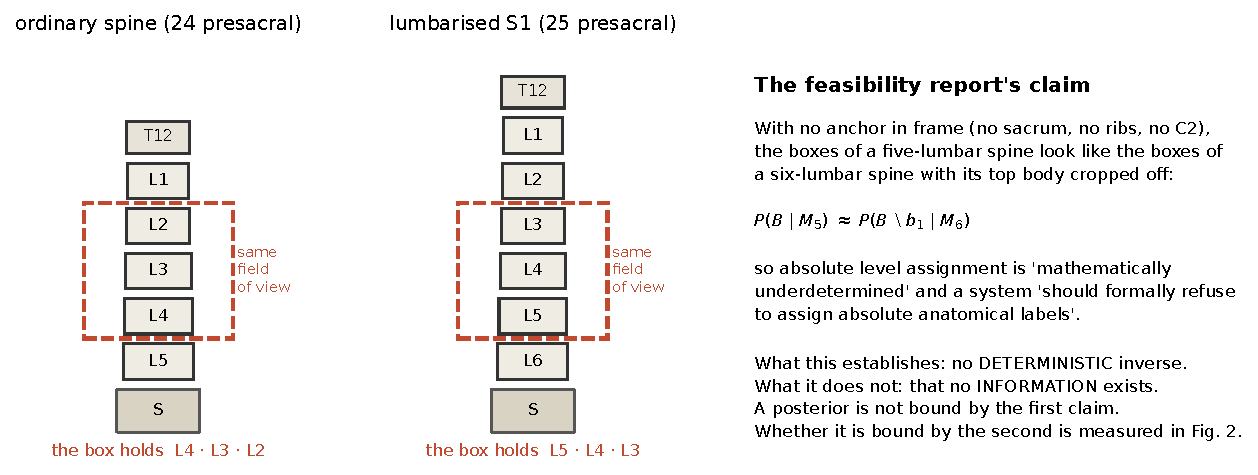
\includegraphics[width=\textwidth]{fig1_problem.pdf}
\caption{One limited field, two spines. The same three-body field holds L4, L3 and L2 in an ordinary spine and L5, L4 and L3 in one with a lumbarised S1, and the boxes are identical. In a limited field the count of a body from the sacrum is undetermined, not merely hard.}
\label{fig:problem}
\end{figure}

\begin{figure}[p]\centering
\includegraphics[width=\textwidth]{fig2_pipeline.pdf}
\caption{The processing chain. One lateral C-arm sweep is exposed up the spine; a detector (shaded, the only learned stage) finds vertebral bodies and the anchor; consecutive frames are linked by normalised cross-correlation; the links form one chain and one panorama; each node's level is its integer count from the anchor; an instrument frame matched onto the chain reads its level.}
\label{fig:pipeline}
\end{figure}

\begin{figure}[p]\centering
\includegraphics[width=\textwidth]{fig3_panorama.pdf}
\caption{Whole-column panorama as the chain builds it on a prone patient, head left, posterior up. Linking consecutive fields numbers every body outward from the sacral anchor, 0 through 23. The count is a position, not a name: no vertebra is identified by it.}
\label{fig:panorama}
\end{figure}

\begin{figure}[p]\centering
\includegraphics[width=\textwidth]{fig4_confirm.pdf}
\caption{Confirmation on a real render. (a) An instrument rests on a vertebra in a limited field. (b) The frame is matched along the full-spine chain and the body it lands on is counted from the sacrum: body 4, L2. (c) Correlation against offset; the margin over the peaks one body off is 0.18. (d) The mechanism.}
\label{fig:confirm}
\end{figure}

\begin{figure}[p]\centering
\includegraphics[width=\textwidth]{fig5_confirm_fluoro.pdf}
\caption{Confirmation on frames formed with a fitted film-noise model, on a spine with a sixth lumbar vertebra. The instrument rests on the body above the sacrum; matched onto the chain it is counted as body 1, L6, truth L6. Margin over the peak one body off 0.37.}
\label{fig:confirmfluoro}
\end{figure}

\begin{figure}[p]\centering
\includegraphics[width=\textwidth]{fig6_arch.pdf}
\caption{The two networks. Top: a stock YOLO11m detector finds every vertebral body in one exposure and names only three classes. Bottom: each detected body becomes one two-channel crop, a ResNet-18 embeds it, and a two-layer bidirectional GRU runs over the sequence of bodies in the frame; the recurrence is the horizontal links between cells, which a per-crop classifier lacks.}
\label{fig:arch}
\end{figure}

\begin{table}[p]\centering\small
\caption{X-ray datasets. Generated from the data manifest, the device cards and the header census (tools/rsnai\_table1.py).}
\label{tab:data}
\resizebox{\textwidth}{!}{% GENERATED by tools/rsnai_table1.py
\begin{tabular}{llllllll}
\toprule
Dataset & C-arm / detector & Pitch (mm) & Stored & kVp & Frames / subjects & Paired with & Licence \\
\midrule
DeepFluoro & Siemens Cios Fusion (csi fpd) & 0.194 & log display & — & 366 frames, 6 cadaveric pelves & CT + C-arm pose per frame & CC BY-NC-SA 4.0 \\
C-ArmLSpine & surgio b51 & 0.15 (307.2 mm / 2048; header PixelSpacing is a 1.0 placeholder) &  & 73--111 & 296 AP + lateral frames, 148 cases (+ 2 raw sweeps) & CBCT per case; pose by registration & CC BY 4.0 \\
COBRA2026, Elekta & Elekta XVI kV imager (four European centres A-D) (unknown fpd) & 0.8 & linear & 120--120 & projection sweeps, 152 cases downloaded of 692 public & planning CT (deformably registered) + RTK geometry & CC BY-NC 4.0 \\
COBRA2026, Varian & — & — & — & — & 26 cases fetched before the analysis (centres F 14, G 12) & planning CT + RTK geometry & CC BY-NC 4.0 \\
Geneva hip & Philips BV Pulsera (ii) & 0.2904 & linear & 65--90 & 116 frames, 19 poses, resin phantom & CT + gold-standard pose & CC BY-SA 4.0 (repository) \\
Ljubljana 2D-3D-GS & Trixell (Ljubljana 2D-3D-GS) PIXIUM 4600 flat panel, fixed radiograph on a turntable (not a C-arm) (csi fpd) & 0.286 & linear & — & 18 frames, cadaver L1--L5 & CT + gold-standard pose & CC BY-NC-ND \\
SpineSAC & — & — & — & — & raw frames of a sawbone phantom on six C-arms & phantom CT + shipped poses; no bone truth yet & — \\
Plain-film corpora & — & — & — & — & CSXA 4,963; BUU-LSPINE 3,603 LA + 3,600 AP; NHANES II 17,073 films (543 with landmarks); VinDr-SpineXR 10,466 images / 5,000 studies (none in the level bank); AASCE 457; Mendeley 714 (excluded: BUU redistribution) & keypoint / level labels & per source \\
FluoroCap panels & — & — & — & — & 29,484 literature fluoroscopy panels (unpaired) & none & figure reuse only \\
\bottomrule
\end{tabular}
}
\end{table}

\bibliographystyle{unsrtnat}
\bibliography{refs}
\end{document}
